\hypertarget{group__inv__clarke}{}\section{Vector Inverse Clarke Transform}
\label{group__inv__clarke}\index{Vector Inverse Clarke Transform@{Vector Inverse Clarke Transform}}
Collaboration diagram for Vector Inverse Clarke Transform\+:
\nopagebreak
\begin{figure}[H]
\begin{center}
\leavevmode
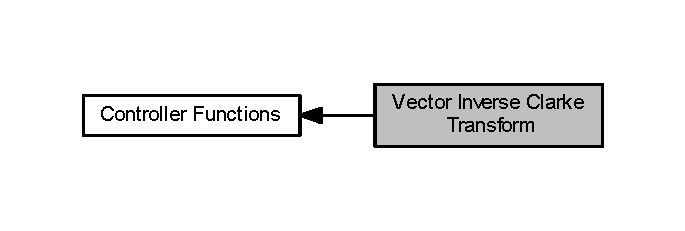
\includegraphics[width=329pt]{group__inv__clarke}
\end{center}
\end{figure}


\subsection{Detailed Description}
Inverse Clarke transform converts the two-\/coordinate time invariant vector into instantaneous stator phases.

The function operates on a single sample of data and each call to the function returns the processed output. The library provides separate functions for Q31 and floating-\/point data types. \begin{DoxyParagraph}{Algorithm}
 where {\ttfamily p\+Ia} and {\ttfamily p\+Ib} are the instantaneous stator phases and {\ttfamily Ialpha} and {\ttfamily Ibeta} are the two coordinates of time invariant vector. 
\end{DoxyParagraph}
\begin{DoxyParagraph}{Fixed-\/\+Point Behavior}
Care must be taken when using the Q31 version of the Clarke transform. In particular, the overflow and saturation behavior of the accumulator used must be considered. Refer to the function specific documentation below for usage guidelines. 
\end{DoxyParagraph}
